\documentclass{article}
\usepackage{fontspec}
\usepackage{polyglossia}
\setdefaultlanguage{french}
\usepackage[a4paper,margin=1.5cm]{geometry}

\usepackage{amsmath}
\usepackage{array}
\usepackage{auto-pst-pdf}
\usepackage{booktabs}
\usepackage{cite}
\usepackage{graphicx}
\usepackage{lmodern}
\usepackage{marvosym}
\usepackage{mathrsfs}
\usepackage{minted}
\usepackage{multicol}
\usepackage{multirow}
\usepackage{paralist}
\usepackage{schemabloc}
\usepackage{siunitx}
\usepackage{soul}
\usepackage{tikz}
\usepackage[european,cuteinductors,siunitx]{circuitikz}
\usepackage{url,hyperref}
\usepackage{verbatim}
\usepackage{xunicode,xltxtra}

\title{
\includegraphics{../../../images/inp-enseeiht} \\ ~ \\ ~ \\ ~ \\ ~ \\ ~ \\ Traitement numérique du signal: \\ ~ \\ Filtrage Multi-Bandes \\ ~}
\author{François Pierron, Guilhem Saurel}
\date{\oldstylenums{\today}}

\begin{document}

\begin{titlepage}
    \setcounter{page}{0}
    \maketitle
    \thispagestyle{empty}

    ~

    ~

    ~
    \tableofcontents
\end{titlepage}


\section{Objectif}

On souhaite synthétiser un filtre dont les spécifications friéquentielles ont plusieurs bandes passantes et coupées :

\begin{tabular}{lrlrl}
    1\textsuperscript{ère} bande coupée:   &    0 < & < ~200 \si\hertz & -30 dB &  \\
    1\textsuperscript{ère} bande passante: &  500 < & < ~400 \si\hertz &   0 dB & tolérance 3dB \\
    2\textsuperscript{ème} bande coupée:   & 1000 < & < 1300 \si\hertz & -30 dB &  \\
    2\textsuperscript{ème} bande passante: & 1500 < & <           Fe/2 &   0 dB & tolérance 3dB \\
\end{tabular}

\section{RIF}

\inputminted[linenos,lastline=21]{matlab}{RIF.m}
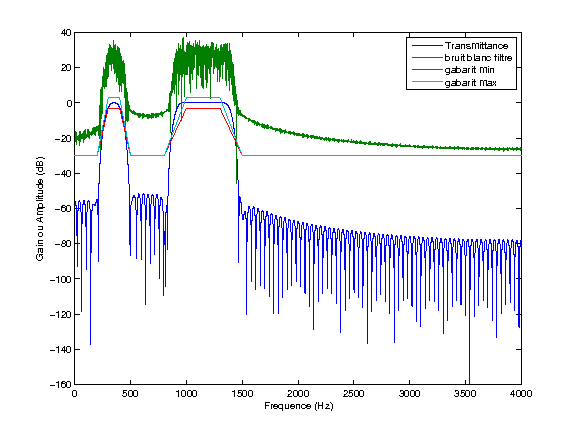
\includegraphics[height=13cm]{RIF_1}
\inputminted[linenos,firstnumber=25,firstline=25,lastline=25]{matlab}{RIF.m}
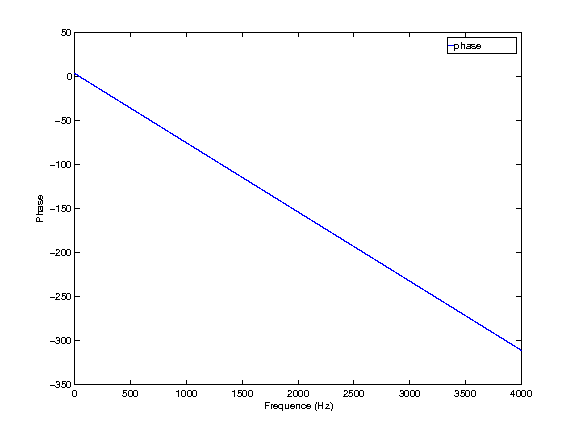
\includegraphics[height=9cm]{RIF_2}\\
NB: On observe bien la linéarité, (contrairement aux filtres RII).\\
\inputminted[linenos,firstnumber=30,firstline=30,lastline=36]{matlab}{RIF.m}
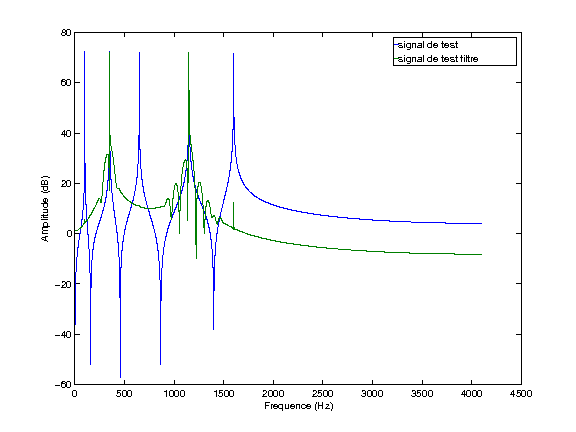
\includegraphics[height=12cm]{RIF_3}

\section{RII}
\subsection{Butterworth}

\inputminted[linenos,lastline=25]{matlab}{RII_butter.m}
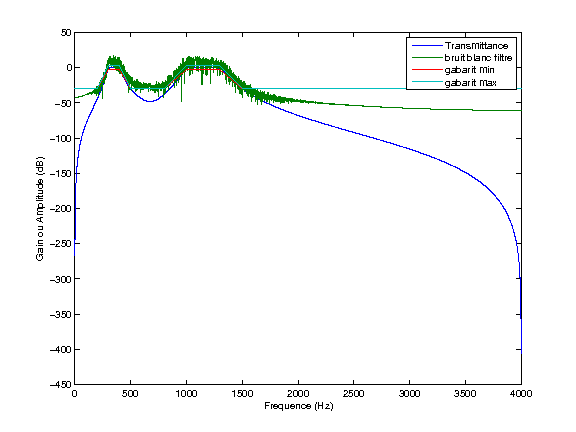
\includegraphics[height=13cm]{butt_1}
\inputminted[linenos,firstnumber=29,firstline=29,lastline=29]{matlab}{RII_butter.m}
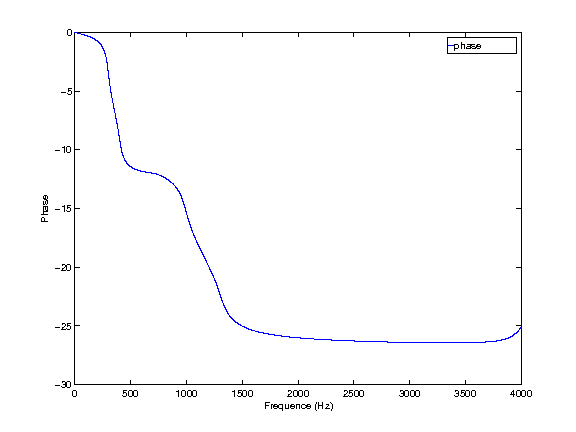
\includegraphics[height=9cm]{butt_2}
\inputminted[linenos,firstnumber=34,firstline=34,lastline=43]{matlab}{RII_butter.m}
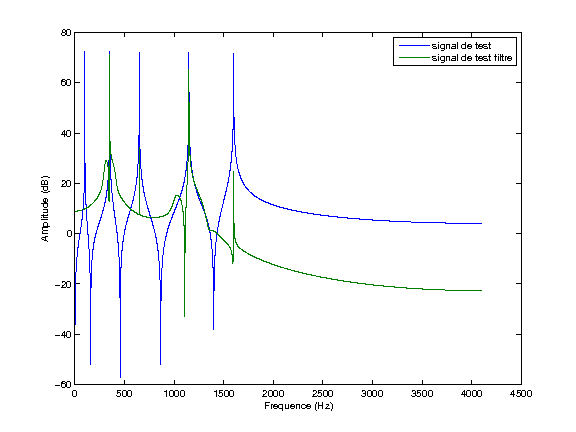
\includegraphics[height=13cm]{butt_3}

\subsection{Chebycheff 1}

\inputminted[linenos,lastline=25]{matlab}{RII_Cheby1m.m}
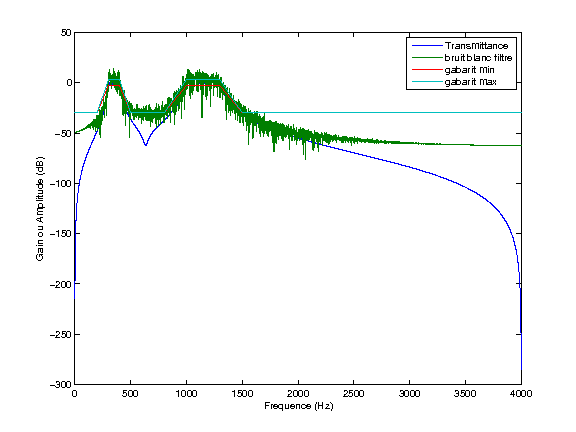
\includegraphics[height=13cm]{cheb1_1}
\inputminted[linenos,firstnumber=29,firstline=29,lastline=29]{matlab}{RII_Cheby1m.m}
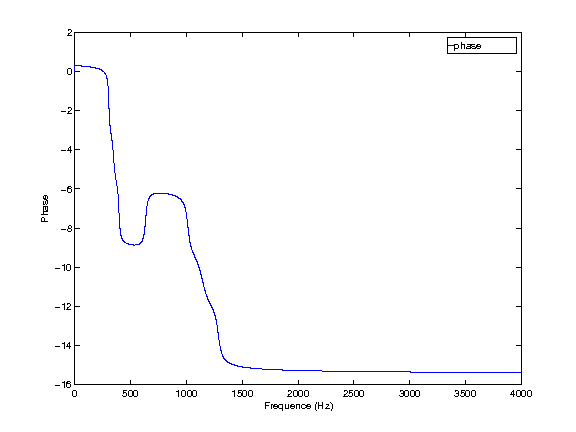
\includegraphics[height=9cm]{cheb1_2}
\inputminted[linenos,firstnumber=34,firstline=34,lastline=42]{matlab}{RII_Cheby1m.m}
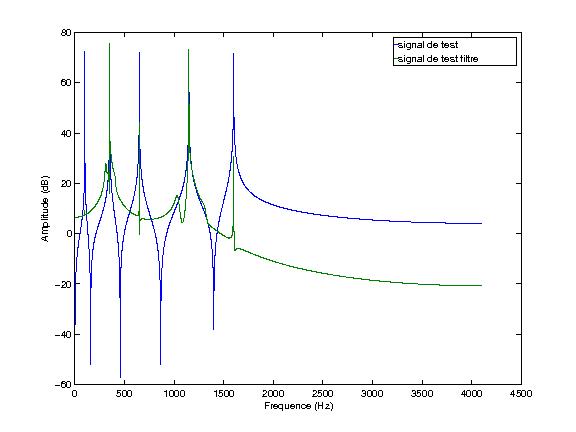
\includegraphics[height=13cm]{cheb1_3}

\subsection{Chebycheff 2}

\inputminted[linenos,lastline=25]{matlab}{RII_Cheby2.m}
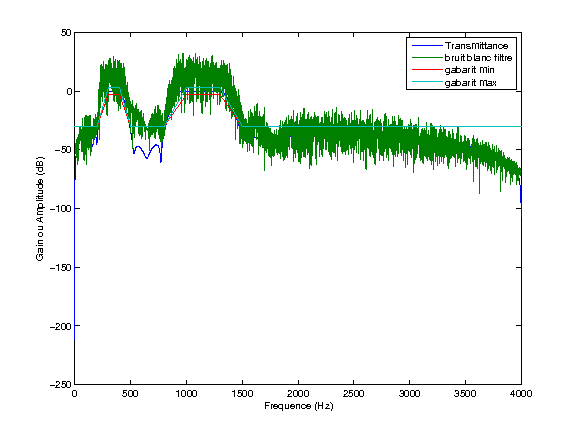
\includegraphics[height=13cm]{cheb2_1}
\inputminted[linenos,firstnumber=29,firstline=29,lastline=29]{matlab}{RII_Cheby2.m}
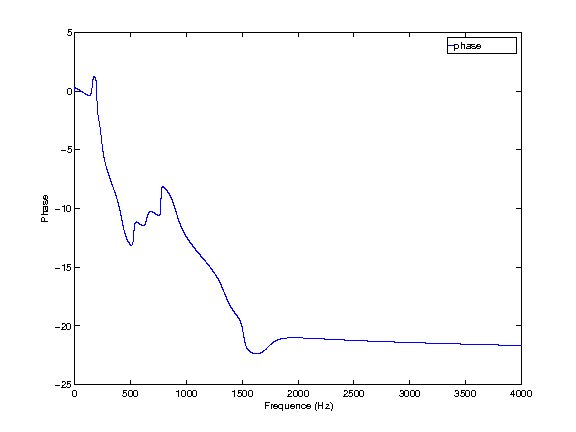
\includegraphics[height=9cm]{cheb2_2}
\inputminted[linenos,firstnumber=34,firstline=34,lastline=42]{matlab}{RII_Cheby2.m}
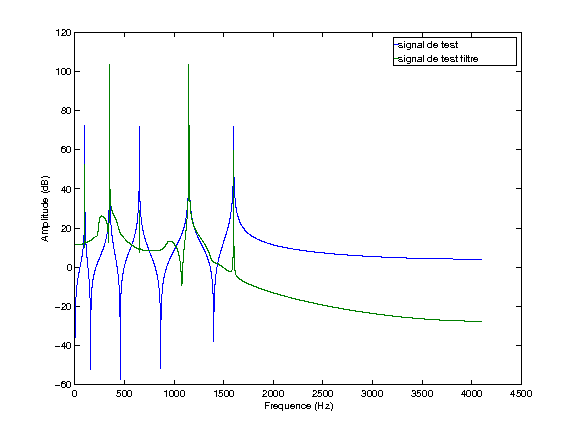
\includegraphics[height=13cm]{cheb2_3}

\subsection{Elliptique}

\inputminted[linenos,lastline=25]{matlab}{RII_ellip.m}
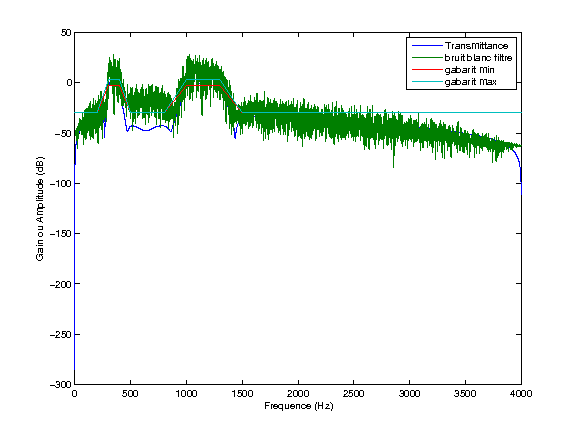
\includegraphics[height=13cm]{ell_1}
\inputminted[linenos,firstnumber=29,firstline=29,lastline=29]{matlab}{RII_ellip.m}
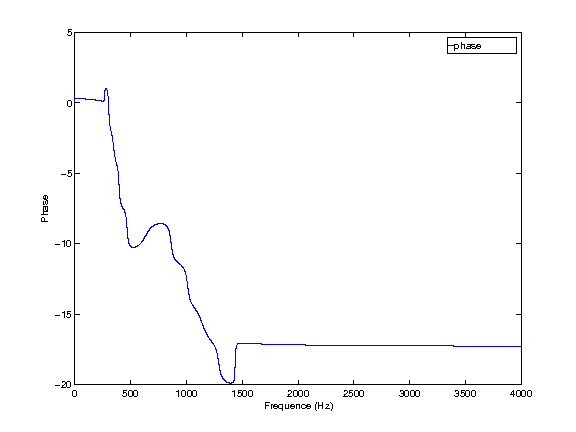
\includegraphics[height=9cm]{ell_2}
\inputminted[linenos,firstnumber=34,firstline=34,lastline=43]{matlab}{RII_ellip.m}
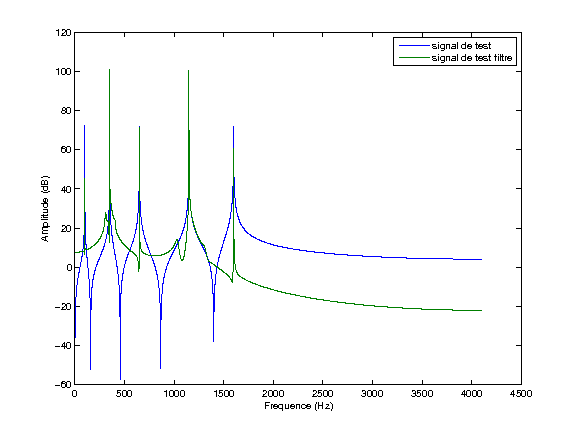
\includegraphics[height=13cm]{ell_3}

\end{document}

